\documentclass[10pt,paper=letter]{scrartcl}
\usepackage[alttitle]{cjquines}

\begin{document}

\title{VCSMS PRIME}
\subtitle{Program for Inducing Mathematical Excellence}
\author{Week 2 Homework}
\date{Due September 27, 2017}

\maketitle
\setlength{\unitlength}{1in}
\begin{picture}(0,0)
  \put(5.5,0.5){\hbox{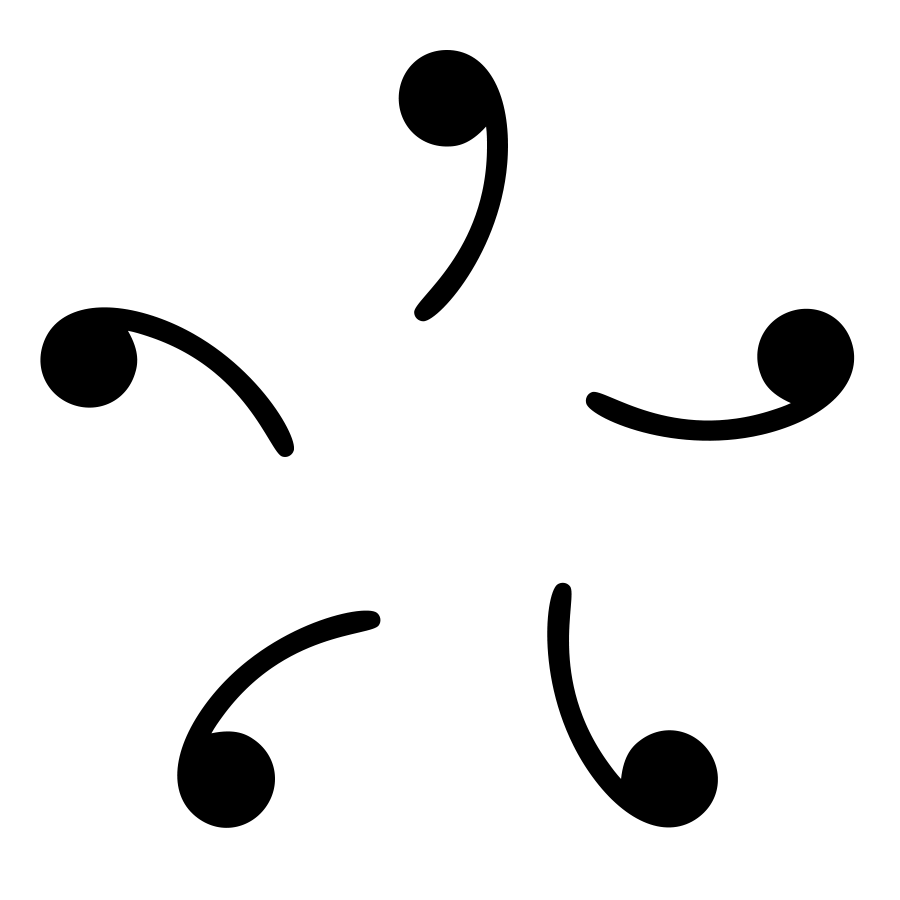
\includegraphics[width=0.9in]{logo.png}}}
\end{picture}
\vspace{-3.5em}

\subsubsection*{Homework}

Due on Wednesday, September 27. Reminder: you can always ask me or your classmates for help, it's okay!

\begin{description}
  \item [Set A] (13) \textbf{S4}: Ad hoc 2; Inclusion-Exclusion 1--2, 4; Permutations 1--2; Combinations 1; Balls and urns 1--2. \textbf{S6}: Random variable 1--2; Random selection 1--2.
  \item [Set B] (13) \textbf{S4}: Ad hoc 3; Inclusion-Exclusion 3, 5; Permutations 3--4; Combinations 2; Balls and urns 3--4. \textbf{S6}: Random selection 3--5; Geometric probability 1; Existence combinatorics 1.
  \item [Set C] (13) \textbf{S4}: Ad hoc 5; Permutations 5, 8; Combinations 3; Balls and urns 5--6.\\\textbf{S6}: Random variable 3; Random selection 6--8; Geometric probability 2--3; Existence combinatorics 2.
  \item [Set D] (13) \textbf{S4}: Ad hoc 10; Permutations 6--7; Balls and urns 7.\\\textbf{S6}: Random variable 4; Random selection 9; Geometric probability 4; Existence combinatorics 3--8.
\end{description}

\subsubsection*{Additional problems}

Reminder: if you want more problems for practice I have some to give, just name a topic. This one includes some topics that haven't appeared in past PMOs but can appear in the future. 

\begin{enumerate}
  \item (AIME II 2004/4) How many positive integers less than 10,000 have at most two different digits?

  \item (OMO Winter 2012/2) How many ways are there to arrange the letters AAAHH so that the sequence HA appears at least once?

  \item (OMO Spring 2015/6) We delete the four corners of an $8\times 8$ chessboard. How many ways are there to place eight non-attacking rooks on the remaining squares?

  \item (AIME I 2001/6) A fair die is rolled four times. What is the probability each of the final three rolls is at least as large as the roll preceding it?

  \item (AIME I 2008/11) Consider sequences that consist entirely of $A$s and $B$s such that every run of consecutive $A$s has even length, and every run of consecutive $B$s has odd length. Examples are $AA$, $B$, and $AABAA$, while $BBAB$ is not such a sequence. How many such sequences have length $14$?

  \item (SASMO 2015) Cheryl gives Albert and Bernard a list of 10 possible dates for her birthday: May 15, 16, 19; June 17, 18; July 14, 16; and August 14, 15, 17. Cheryl tells Albert the month of her birthday, and tells Bernard the day of her birthday. Given the following conversation, when is Cheryl's birthday?

  Albert: ``I don't know when Cheryl's birthday is, but I know that you don't know either.''

  Bernard: ``At first I didn't know when Cheryl's birthday is, but now I know.''

  Albert: ``Now I also know when Cheryl's birthday is.'' 

  \item (AMC 12A 2007/25) Call a set of integers \emph{spacy} if it contains no more than one out of any three consecutive integers. How many subsets of $\{1, 2, 3, \ldots, 12\}$, including the empty set, are spacy?

  \item (AIME 1986/13) How many different sequnces of $15$ coin tosses contain exactly two pairs of consecutive heads, three pairs of consecutive heads then tails, four pairs of consecutive tails then heads and five pairs of consecutive tails?

\end{enumerate}

\end{document}
